\begin{figure}
\centering
\vphantom{7cm}
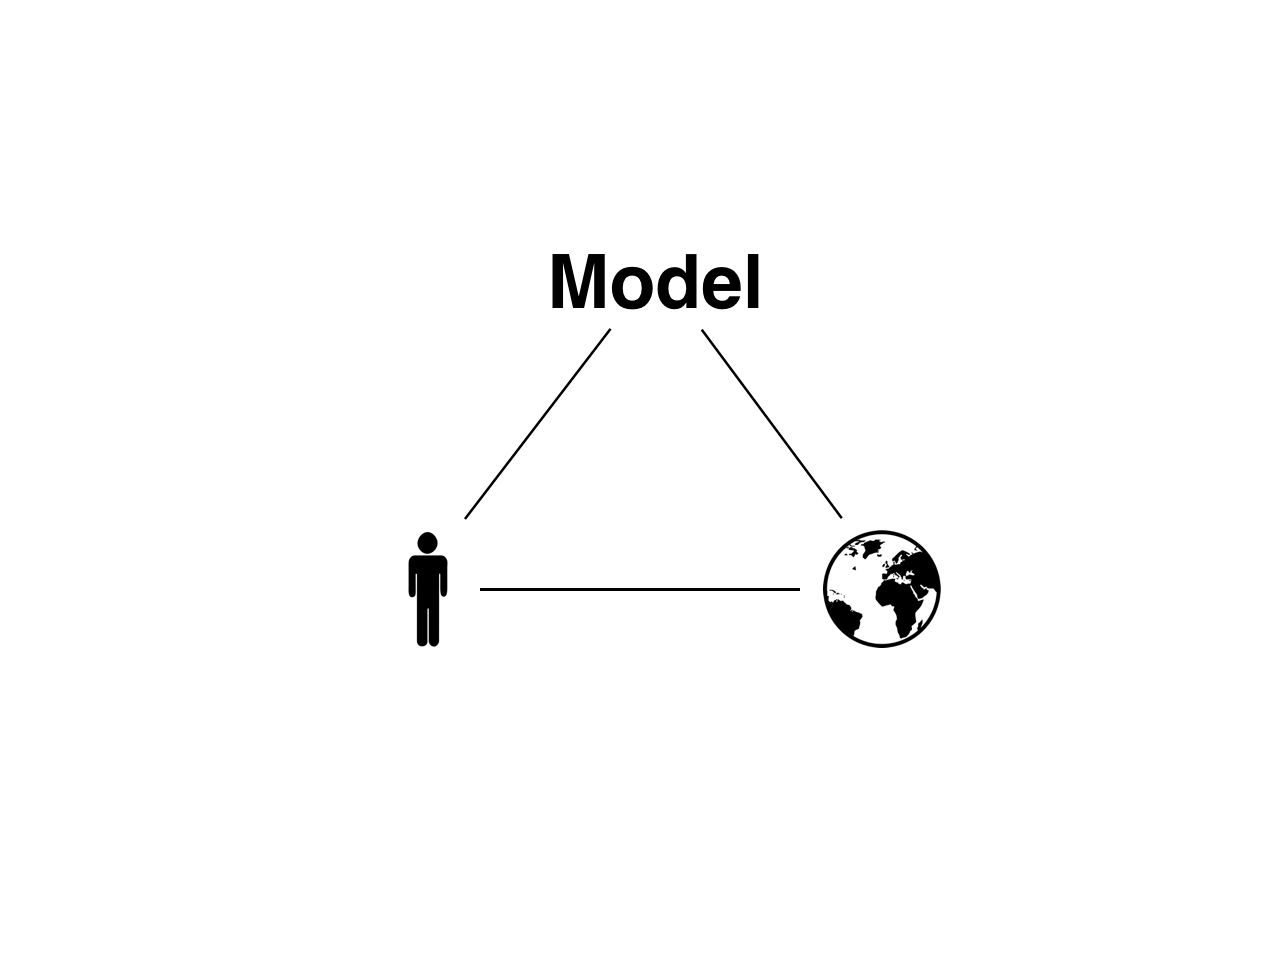
\includegraphics[trim={7cm 8cm 7cm 8cm},clip=true,width=0.275\linewidth]{figs/motivation/hmr}
~
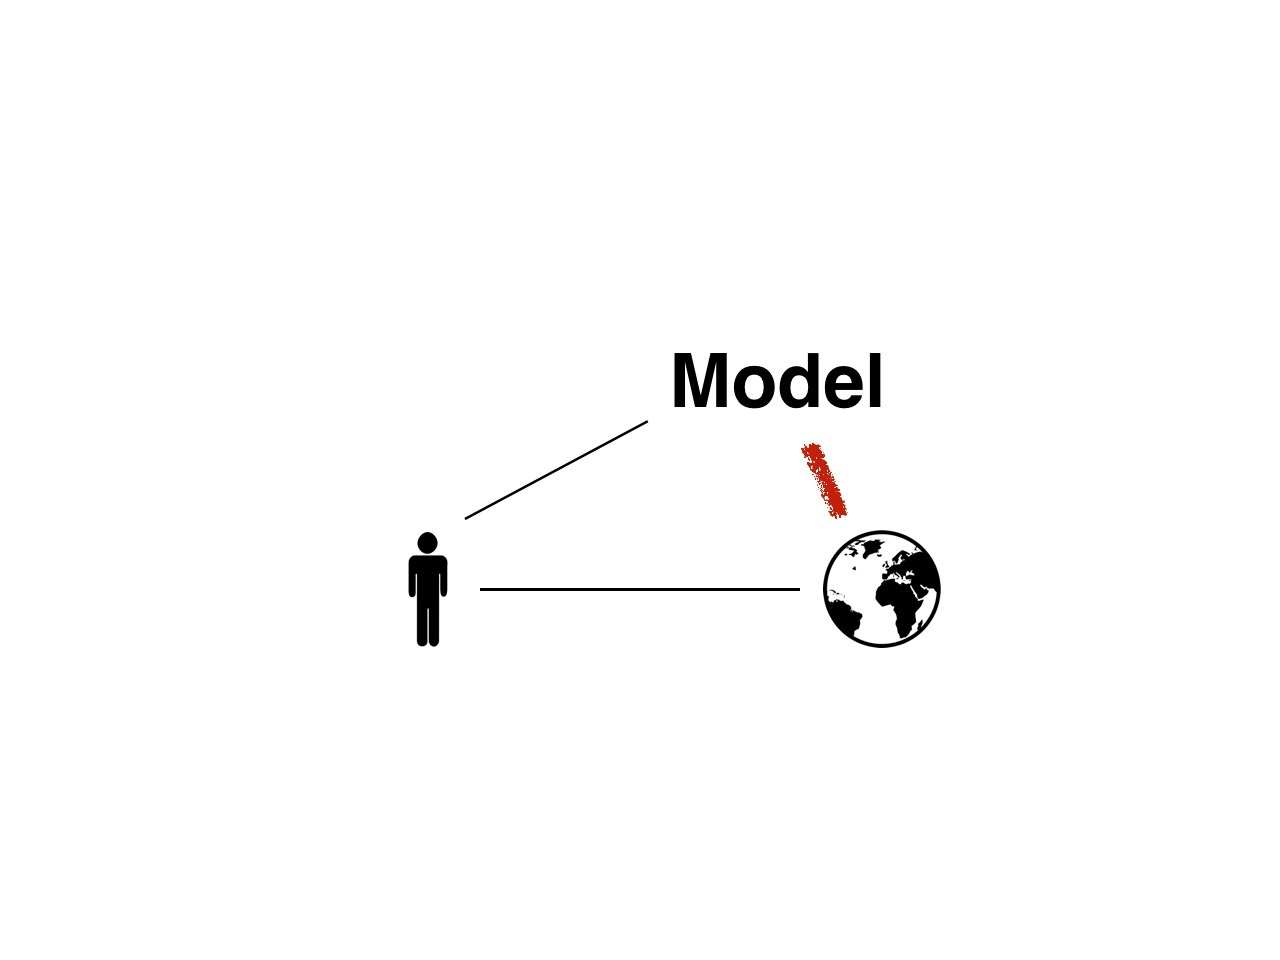
\includegraphics[trim={7cm 8cm 7cm 8cm},clip=true,width=0.275\linewidth]{figs/motivation/hmr_complex}
~
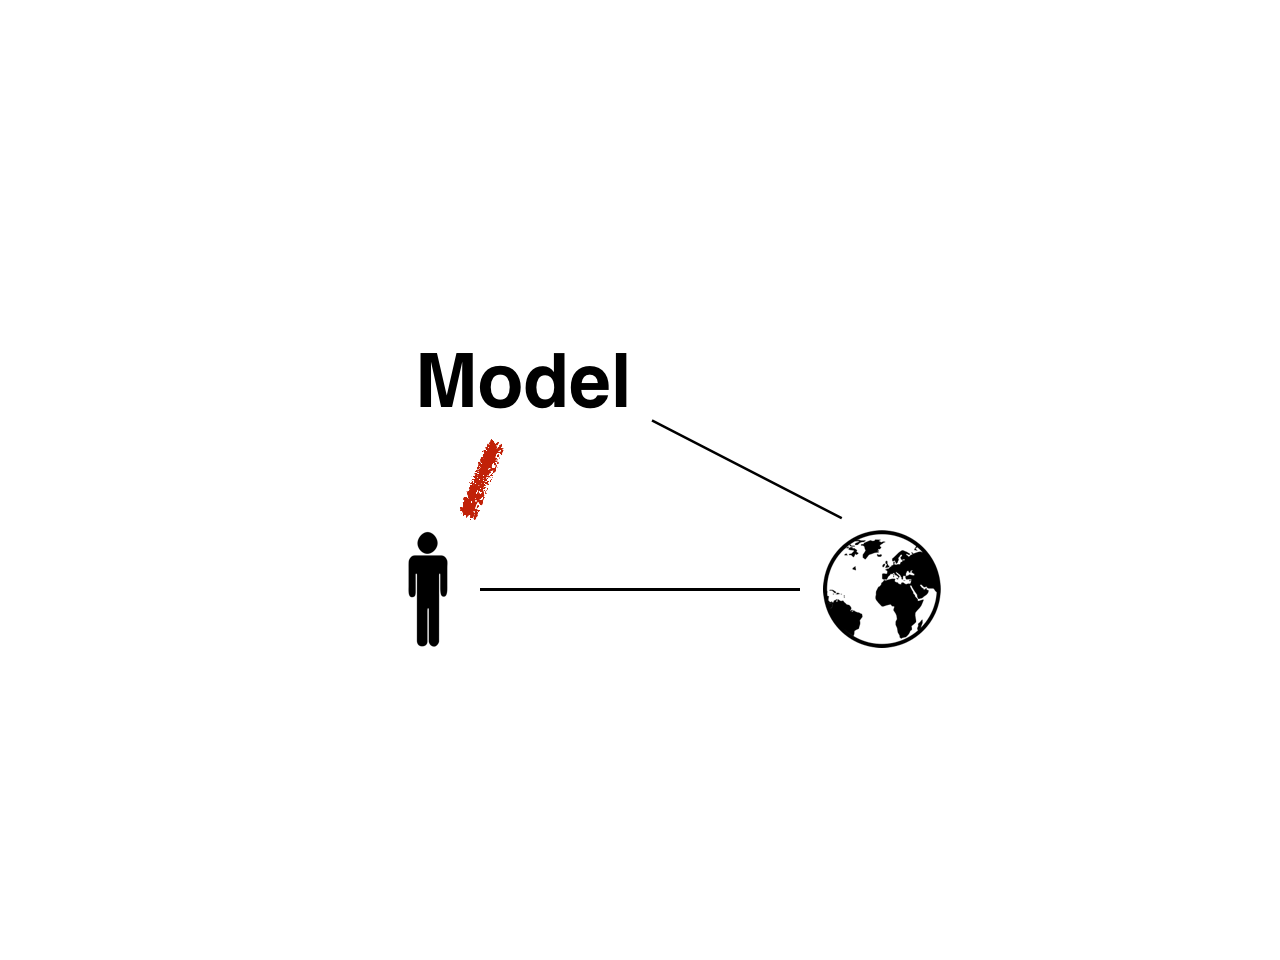
\includegraphics[trim={7cm 8cm 7cm 8cm},clip=true,width=0.275\linewidth]{figs/motivation/hmr_interpretable}
\caption{
Humans (lower left) build machine learning models (top) to understand and
predict reality (lower right). The second image illustrates how improving
machine learning models (ie., closing the gap between the model and reality)
makes it harder for humans to understand it. Likewise, simplifying the model
(ie., closing the gap between the model and the human) makes the model less
accurate (third image).
}
\label{figs:motivation_hmr}
\end{figure}